\section{Concentration Without Independence}
This chapter mainly explores other approaches to concentration that do not rely on independence.



% ----------5.1----------
\subsection{Cencentration of Lipschitz Functions on the Sphere}
For a random vector $X$ in $\mathbb{R}^n$ and a function $f: \mathbb{R}^n \to \mathbb{R}$. When does the 
random variable $f(X)$ concentrate, i.e.
\[ f(X) \approx \mathbb{E}[f(X)] \text{ with high probability? } \]
If $X$ is normal and $f$ is linear, this is easy: $f(X)$ is normal (\cref{cor:3.3.2}) and concentrates well 
(\cref{prop:2.1.2}).

What about for general \textit{nonlinear} functions $f$? We can't expect good concentration for any $f$, 
but if $f$ does not oscillate too wildly, we might get good concentration. Namely, we'll use Lipschitz 
functions to rule out these oscillations:


\subsubsection{Lipschitz Functions}
\begin{definition}[]
\label{def:5.1.1}
Let $(X, d_X)$ and $(Y, d_Y)$ be metric spaces. A function $f:X \to Y$ is called \underline{Lipschitz} if 
there exists $L \in \mathbb{R}$ such that 
\[ d_Y(f(u), f(v)) \leq L \cdot d_X(u, v) \text{ for every } u, v \in X. \]

The infimum of all $L$ in this definition is called the \underline{Lipschitz norm} because of $f$ and is denoted 
$\lVert f \rVert_{\mathrm{Lip}}$.

If $\lVert f \rVert_{\mathrm{Lip}} \leq 1$, $f$ is called a \underline{contraction}.
\end{definition}

(\textbf{Important}) Technically the Lipschits norm is only a seminorm, since it vanishes on nonzero constant 
functions. It's called a norm in the book for brevity.

The class of Lipschitz functions sits between differentiable and uniformly continuous: 
\[ f \text{ is differentiable } \implies f \text{ is Lipschitz } \implies f \text{ if uniformly continuous.} \]

Moreover, from Exercise 5.1,
\[ \lVert F \rVert_{\mathrm{Lip}} \leq \sup_{x \in \mathbb{R}^n} \lVert \nabla f(x) \rVert_{2}. \]

\begin{example}[]
\label{ex:5.1.2}
Vectors, matries, and norms define natural Lipschitz functions:
\begin{enumerate}
	\item For a fixed vector $\theta \in \mathbb{R}^n$, the linear functional 
	\[ f(x) = \left\langle x, \theta \right\rangle \text{ has Lipschitz norm } 
	\lVert f \rVert_{\mathrm{Lip}} = \lVert \theta \rVert_{2}. \]
	\item More generally, any $m \times n$ matrix $A$, the linear operator 
	\[ f(x) = Ax \text{ has Lipschitz norm } \lVert F \rVert_{\mathrm{Lip}} = \lVert A \rVert_{}. \]
	\item For any norm $\lVert \cdot \rVert_{}$ on $\mathbb{R}^n$, the function 
	\[ f(x) = \lVert x \rVert_{} \]
	has Lipschitz norm equal to the smallest $L$ such that 
	\[ \lVert x \rVert_{} \leq L \lVert x \rVert_{2} \text{ for all } x \in \mathbb{R}^n. \]
\end{enumerate}
\end{example}

\begin{proof}
Exercise 5.2.
\end{proof}


\subsubsection{Concentration via Isoperimetric Inequalities}
Any Lipschitz function on the Euclidean sphere $S^{n - 1} = \{x \in \mathbb{R}^n: \ \lVert x \rVert_{2} = 1\}$ 
concentrates:

\begin{theorem}[]
\label{thm:5.1.3}
Let $X \sim \mathrm{Unif}(\sqrt{n}S^{n - 1})$. Then for any Lipschitz function $f: \sqrt{n}S^{n - 1} \to 
\mathbb{R}$ we have 
\[ \lVert f(X) - \mathbb{E}[f(X)] \rVert_{\psi_2} \leq C \lVert f \rVert_{\mathrm{Lip}}. \]
\end{theorem}

The theorem above works for the geodesic distance metric as well (Exercise 5.4).

\cref{thm:5.1.3} has been proved already for linear functions $f$. \cref{thm:3.4.5} tells us that $X$ is a 
subgaussian random vectos, and this by definition means that any lienar function of $X$ is a subgaussian 
random variable. 

To fully prove \cref{thm:5.1.3}, we need to argue that any Lipschitz function concentrates at least as well 
as a linear function. We'll use the aread of their \underline{sublevel sets} - regions of the sphere where 
$f(x) \leq a$ for a given level $a$. To do this, we'll use the \textit{isoperimetric inequality}, namely 
the one for subsets on $\mathbb{R}^n$: 

\begin{theorem}[Isoperimetric inequality on $\mathbb{R}^n$]
\label{thm:5.1.4}
Among all subsets $a \subset \mathbb{R}^n$ with given volume, the Euclidean balls have minimal area. Moreover, 
for any $\varepsilon > 0$, the Euclidean balls minimize the volume of the $\varepsilon$-neighborhood of $A$, 
defined as 
\[ A_{\varepsilon} = \{ x \in \mathbb{R}^n: \ \exists y \in A \text{ such that } \lVert x - y \rVert_{2} 
\leq \varepsilon \} = A + \varepsilon B_2^n. \] 
The figure below illustrates the isoperimetric inequality:
\begin{center}
	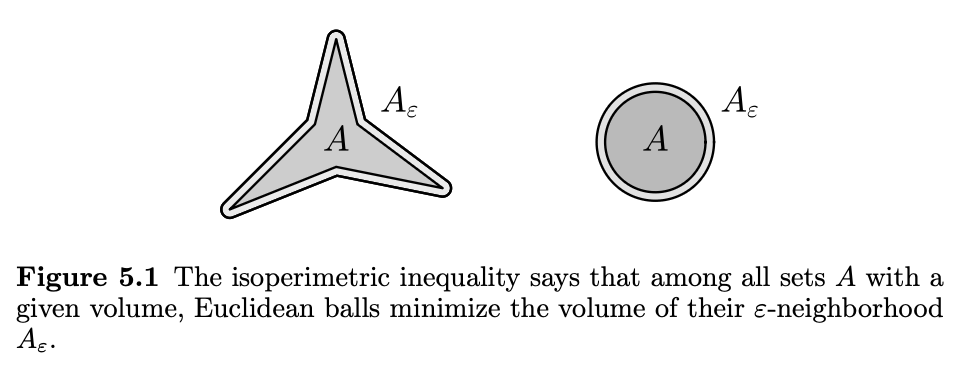
\includegraphics[width=0.8\textwidth]{Chapter 5/fig5-1.png}
\end{center}
\end{theorem}

A similar isoperimetric inequality holds for subsets on $S^{n - 1}$, and in this case the minimizers are the 
\underline{spherical caps} - neighborhoods of a single point. To state this principle, let $\sigma_{n - 1}$ 
denote the normalized are on the sphere $S^{n - 1}$ (The $n - 1$-dimensional Lebesgue measure).

\begin{theorem}[Isoperimetric inequality on the sphere]
\label{thm:5.1.5}
Let $\varepsilon > 0$. Then among all subsets $A \subset S^{n - 1}$ with given area $\sigma_{n - 1}(A)$, the 
spherical caps minimizer the area of the neighborhood $\sigma_{n - 1}(A_{\varepsilon})$, where 
\[ A_{\varepsilon} := \{ x \in \mathbb{R}^n: \ \exists y \in S^{n - 1} \text{ such that } 
\lVert x - y \rVert_{2} \leq \varepsilon \}. \]
\end{theorem}


\subsubsection{Blow-up of Sets on the Sphere}
The isoperimetric inequality leads to a remarkable and counterintuitive result: if a set $A$ covers at least 
half of the sphere in area, its $\varepsilon$-neighborhood $A_{\varepsilon}$ will cover most of the sphere. 
To simplify things in view of \cref{thm:5.1.3}, we'll operate on the sphere with radius $\sqrt{n}$.

\begin{lemma}[Blow-up]
\label{lem:5.1.6}
Let $A \subset \sqrt{n}S^{n - 1}$, and let $\sigma$ denote the normalized are on that sphere. If 
$\sigma(A) \geq 1/2$, then for every $t \geq 0$, 
\[ \sigma(A_t) \geq 1 - 2 \exp{(-ct^2)}. \]
\end{lemma}

\begin{proof}
Consider the hemisphere defined by the first coordinate:
\[ H := \{x \in \sqrt{n}S^{n - 1}: \ x_1 \leq 0 \}. \]
By assumption, $\sigma(A) \geq 1/2 = \sigma(H)$, hence the isoperimetric inequality (\cref{thm:5.1.5}) implies 
that 
\[ \sigma(A_t) \geq \sigma(H_t). \]
The neighborhood $H_t$ of the hemisphere $H$ is a spherical cap, and we could compute its area directly, but 
it is easier to use \cref{thm:3.4.5} instead, which states that a random vector $X \sim \mathrm{Unif}
(\sqrt{n}S^{n - 1})$ is subgaussian, and $\lVert X \rVert_{\psi_2} \leq C$. Since $\sigma$ is the uniform 
probability measure on the sphere, it follows that 
\[ \sigma(H_t) = P(X \in H_t). \]
Now, the definition of the neighborhood implies that 
\[ \{ x \in \sqrt{n}S^{n - 1}: \ x_1 \leq t / \sqrt{2} \} \subset H_t. \]
Thus
\[ \sigma(H_t) \geq P(X_1 \leq t / \sqrt{2}) \geq 1 - 2 \exp{(-ct^2)}. \]
The last inequality holds because $\lVert X_1 \rVert_{\psi_2} \leq \lVert X \rVert_{\psi_2} \leq C$. Then the 
lemma is proved because $\sigma(A_t) \geq \sigma(H_t)$.
\end{proof}

\begin{remark}[A more dramatic blow-up]
\label{rmk:5.1.7}
The $1/2$ value for the area in \cref{lem:5.1.6} was arbitrary, and can be replaced with any constant, or even 
an exponentially small quantity (Exercise 5.3)!
\end{remark}

\begin{remark}[A zero-one law]
\label{rmk:5.1.8}
The blow-up phenomenen we just saw can be quite counterintuitive at first. However, this is a typical p
phenomenon in high dimensions. It is similar to \textit{zero-one laws} in probability theory, which basically 
say that events influenced by many random variables tend to have probabilities zero or one.
\end{remark}


\subsubsection{Proof of Theorem 5.1.3}




% ----------5.2----------
\subsection{Concentration on Other Metric Measure Spaces}

